\chapter{Introduction}

Introduction aux essais cliniques.

\section{Du laboratoire au patient}
Lorsqu'on veut mettre un nouveau médicament sur le marché, on a plein de questions \ref{fig:questions}.

\begin{figure}[H]
    \centering
    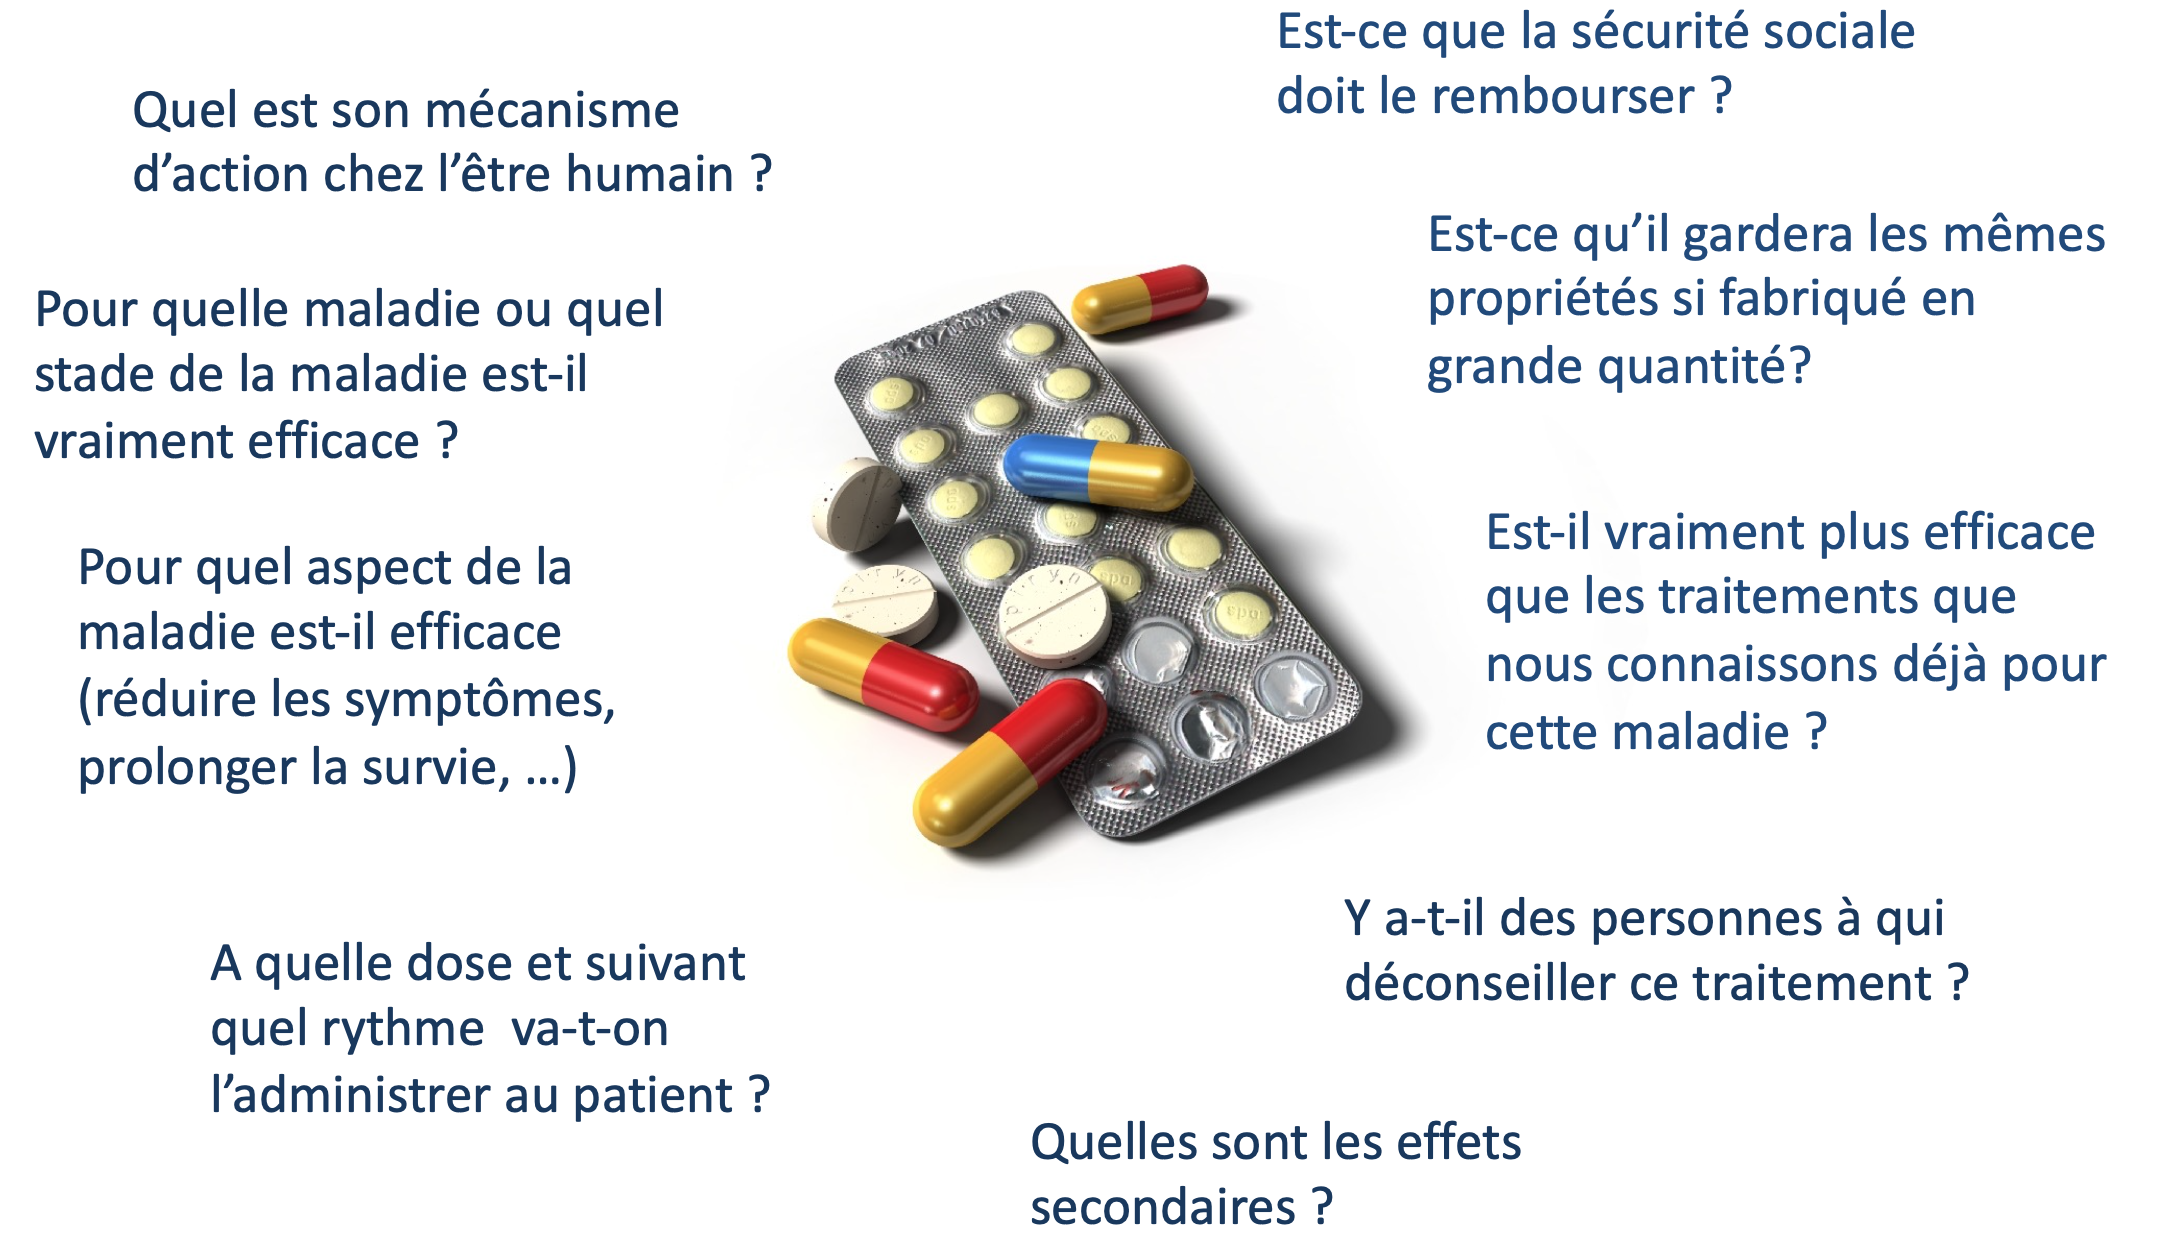
\includegraphics[scale=0.2]{images/questions.png}
    \caption{Questions sur médicament}
    \label{fig:questions}
\end{figure}

La recherche clinique (et préclinique) va tenter d’apporter une réponse à toutes ces questions dans la figure \ref{fig:questions}. La statistique, et plus particulièrement la biostatistique, est un outil fondamental de la recherche clinique.

La recherche clinique se base sur la mise sur pied, la réalisation, l’analyse et la diffusion d’essais cliniques.\\


\textbf{Essai clinique} toute expérience sur des êtres humains visant à déterminer l’impact d’un (ou plusieurs) traitement(s) pour guérir, soigner ou prévenir une maladie.\\

Le plus souvent : Essais cliniques impliquant deux (ou plusieurs) traitements appliqués à deux (ou plusieurs) groupes de personnes ou patients qui sont enrôlés, traités et suivi suivant le même protocole.\\

\textbf{But des essais cliniques :}
\begin{itemize}
    \item Découvrir, étudier et développer de nouveaux traitements pour guérir, soigner ou prévenir une maladie
    \item Fournir suffisamment d’évidence pour changer la pratique clinique dans le traitement d’une maladie spécifique et d’une population spécifique
\end{itemize}

\vspace{0.15cm}
\textbf{ Traitement :}
\begin{itemize}
    \item Un médicament particulier à un certain dosage, une combinaison de médicaments, etc
    \item Une technique chirurgicale, une technique de radiothérapie, etc 
    \item Un régime, des mesures en matière d’hygiène de vie, une
campagne de prévention, etc
    \item Une stratégie de traitements (combinaison de différentes approches)
\end{itemize}


\subsection{Déclaration d’Helsinki}
Cela correspond aux droits du patient. C'est l'énoncé des principes éthiques applicables à la recherche médicale impliquant des êtres humains. Les objectifs de la recherche médicale ne doivent jamais prévaloir sur les droits des personnes impliquées.


\subsection{Comité d’éthique et Consentement éclairé}

Tous les protocoles de recherche impliquant des êtres humains doivent être revus et approuvés par le board institutionnel et le comité d’éthique (CE) avant de pouvoir démarrer. Ces comités restent impliqués tout au long de l'étude et tout événement inattendu arrivant durant le cours d’un essai doivent leur être signalés.\\

Les patients éligibles ne peuvent être enrôlés dans un essai clinique seulement une fois :
\begin{itemize}
    \item qu’ils ont été informés que leur participation n’est pas obligatoire, et qu’une fois enrôlés ils peuvent quitter l’essai à tout moment
    \item qu’ils ont été informés des risques et des bénéfices de leur participation dans l'essai clinique avec suffisamment de détails
    \item qu’ils ont signé un \textbf{consentement éclairé} pour leur participation.

\end{itemize}

\section{Essais Cliniques : principe}
Les différentes étapes sont :
\begin{enumerate}
    \item Protocole : objectif, méthodologie
    \item Sélections des centres, des investigateurs, accord du CE
    \item Sélections et traitement de patients
    \item Encodage des données
    \item Analyse statistiques des données
    \item Publication/présentation des résultats.
\end{enumerate}
\vspace{0.15cm}
Le biostatisticien va jouer un rôle dans plusieurs étapes. Il est impliqué dans la mise en place du protocole, dans l'analyse statistique et dans la publication des résultats. 

\subsection{Effet traitement}
\textbf{L’effet d’un traitement} pour un patient est la différence entre ce qu’il est arrivé au patient suite à l’administration de ce traitement et ce qu’il serait arrivé à ce patient s’il n’avait pas reçu ce traitement. (Senn, 1999)\\

Les points importants sont : 
\begin{itemize}
    \item Idée de comparaison : effet du traitement est toujours comparatif ! \item Effet du traitement 1 Activité du traitement
    \item Notion de CAUSALITÉ !
\end{itemize}
\vspace{0.15cm}
Différents effets peuvent influencer la maladie sans que ce soit le médicament. Il faut les prendre en compte.\\

\begin{itemize}
    \item Cours naturel de la maladie 
    \item \textbf{Facteurs confondant} (exemple Glace-noyade)
    \item Effet de sélection
     \item \textbf{ Régression to the mean} (exemple avec performance extraordinaire et faible probabilité de la répéter)
     \item ...
\end{itemize}
\vspace{0.15cm}
La question importante est \textbf{Comment établir la causalité ?}\\

Pour répondre « OUI » sans ambiguïté, il faut que les deux
groupes soient comparables en tout point : même âge, même
pronostique, même niveau socio-économique, ….

\subsection{Randomisation}
Le choix du traitement est alloué au hasard aux différents patients.\\
\begin{itemize}
    \item Comparaison non biaisée des traitements
    \item Variables confondantes distribuées également entre les groupes
    \item Base de l’inférence statistique
\end{itemize}
\vspace{0.15cm}
\textbf{Principe de base} : randomisation totalement aléatoire\\
\begin{itemize}
    \item Chaque patient à la même chance de recevoir chacun des
traitements étudiés
    \item L’assignement d’un patient à un groupe traitement n’influence pas le choix du traitement des autres patients
    \item On ne sait pas à l’avance quel traitement chacun des patients va recevoir.
\end{itemize}
\vspace{0.15cm}
\textbf{La randomisation des patients entre les différents traitements n’est éthiquement acceptable que :}\\
\begin{itemize}
    \item si le médecin (et de façon générale la communauté scientifique) est en état d’équipoise.

\item si un traitement efficace est connu, mais que les conséquences d’un traitement de contrôle sans traitement sont réversibles et modérées (par exemple mal de tête) et que le ratio risque-bénéfice peut justifier l’essai clinique.
\end{itemize}

\subsection{Réponse (Outcome)}

Les effets du traitement sont évalués en mesurant une ou plusieurs caractéristiques sur les patients = \textbf{variable(s) que l’on va étudier}\\

\textbf{Remarques}\\

\begin{itemize}
    \item Endpoint principal et endpoints secondaires
    \begin{itemize}
        \item  L’\textbf{endpoint principal} sera utilisé pour le calcul de taille
d’échantillon et pour les conclusions principales de l’étude
\item Les \textbf{endpoints secondaires} seront utilisés pour
confirmer/appuyer les conclusions tirées sur base de
l’endpoint principal
    \end{itemize}
\item Le choix de l’endpoint principal (et des endpoints secondaires)
est crucial et doit rencontrer un consensus
\item Uniformisation des mesures pour diminuer la variabilité
\end{itemize}
\vspace{0.15cm}
\textbf{Comment généraliser ces résultats à d’autres patients que ceux dans l’essai clinique ?}\\

On fait des tests cliniques sur un sous groupe de la population et on fait une extrapolation.
\subsection{Extrapolation}
Pour pouvoir faire de l’inférence(=interpolation) il faut que l’échantillon soit :
\begin{itemize}
    \item  En théorie : ALÉATOIRE
    \item En pratique : REPRÉSENTATIF de la population
\end{itemize}
\vspace{0.15cm}
Pour s’assurer de la représentativité de l’échantillon, les patients entrés dans l’essai clinique devrait être un échantillon aléatoire de la population étudiée. Mais Impossible pour des raisons éthiques et pratiques. Les patients entrés dans l’essai clinique doivent être
représentatifs de la population étudiée(problème de sous représentativité des minorités ethniques dans les essais cliniques).\\

\textbf{Si on s’intéresse à l’effet d’un nouveau traitement, peut-on directement commencer un tel essai clinique ?}
 Non on a des phases bien précises à respecter. Ces phases permettent de collecter des informations sur la posologie, la dose, les mécanismes d'action et l'activité du traitement, les effets secondaires, ....
 
 \subsection{Différentes phases}
 \subsubsection{Phases avant expérimentation clinique}
 On a deux phases avant les expérimentations cliniques : \textbf{recherche de base} qui se fait in vitro en laboratoire et \textbf{expérimentation préclinique} qui se fait in vivo dans des animaux.
 
\subsubsection{phase I}

\begin{enumerate}
    \item 1ère administration à des êtres humains 
    \item < 100 patients, 10-30 patients
    \item Action de la molécule ("bio-chimique") 
    \item Profil de toxicité
    \item Dose(s) recommandée(s)
\end{enumerate}

\subsubsection{phase II}

\begin{enumerate}
    \item  1ère évaluation de l’activité chez des êtres humains (en général : affectés par la maladie)
    \item<100 patients, 40-80 patients
    \item Profile de toxicité
    \item Dose
    \item Réponse, mécanisme d’action
\end{enumerate}

\subsubsection{phase III}

\begin{enumerate}
    \item  Évaluation comparative de l’efficacité
    \item Plusieurs centaines/milliers de patients
    \item Toxicité
    \item Efficacité
\end{enumerate}

\subsubsection{phase IV}
\begin{itemize}
    \item Follow-up à long-terme (efficacité et safety) dans des conditions plus proches de la réalité, et a plus grande échelle
    \item « pharmacosurveillance » : Peut permettre de mettre en évidence des effets
secondaires rares
    \item Obtenir des données supplémentaires pour les négociations sur le cout et le remboursement possible
    \item Typiquement plusieurs milliers de patients traités dans des conditions beaucoup moins contrôlées
\end{itemize}
\subsubsection{Remarques}
\begin{itemize}
    \item Plusieurs essais sont en général réalisés pour une même phase. Ces phases ne sont pas toujours aussi distinctes.
    \itemTout au long du processus Phase I-Phase III : les aspects « commerciaux », « techniques », et « marketing » sont évalués en parallèle.
\item Après complétion de la phase III : soumission aux autorités pour autorisation de mise sur le marché
\end{itemize}
\section{Documents}

\subsection{Protocole}

\textbf{Protocole} : Document rédigé et approuvé avant le début de l’étude et ayant pour but de \textbf{standardiser} la façon dont est menée l’étude. Il contient les points suivants :
\begin{itemize}
    \item Motivation de l’étude, connaissances actuelles
\item Objectif(s) - Question(s) d’intérêt clairement définie(s)
 \begin{itemize}
     \item Objectif principal/Objectifs secondaires
     \item Hypothèses statistiques
 \end{itemize}
\item Outcomes/Mesures de réponse
\begin{itemize}
    \item Outcome principal / secondaires
\end{itemize}
\item Définition de la population cible, échantillonnage et taille d’échantillon
\item Phase, design de l’étude, randomisation.
\item Traitements considérés
\begin{itemize}
    \item Informations disponibles sur ce traitement
    \item Mode d’administration, dosage et posologie
\end{itemize}

\item Prise en charge des patients et collecte des
données
\begin{itemize}
    \item Gestion des effets secondaires, réduction des
doses, traitement concomitant, autres soins, …
\item Examens, visites et données à collecter 
\end{itemize}
\item Technique d’analyse des résultats
\begin{itemize}
    \item En fonction des objectifs, du plan d’expérience et
de la variable d’outcome
\item Monitoring statistique de l’essai
\end{itemize}
\item …
\end{itemize}
\vspace{0.15cm}
La population de l'essai clinique se définit dans le protocole sur base d’une liste de critère d’éligibilité (= liste de critères d’inclusion et de non-inclusion permettant de
définir précisément les patients pouvant être randomisés dans
l’essai clinique.)

\subsection{Plan d’analyse Statistique}

Document rédigé et approuvé avant que le statisticien ait accès aux données de l’étude.\\

\begin{itemize}
    \item SAP en anglais (Statistical Analysis Plan)
    \item Peut être une partie du protocole ou un document séparé
    \item A pour but principal d’éviter le « qui cherche trouve » 
     \item Toutes les analyses statistiques prévues doivent être pré- spécifiée dans le SAP. Les analyses non pré-spécifiées dans le SAP seront interprétées comme « exploratoires »
    \item Clairement le type d’analyse dépendra du choix de l’endpoint et des objectifs de l’étude. Ces techniques d’analyse doivent être conformes aux recommandations faites dans les guidelines internationales.
\end{itemize}\\

Ce doucement doit détailler :

\begin{itemize}
    \item Les patients inclus dans chaque analyse (« Intent-toTreat » ou du
«Per-protocol »)
\item Le niveau « d’importance » de chaque analyse (primary,
secondary, supportive, exploratory, …)
\item Les méthodes statistiques utilisées, et notamment
\begin{itemize}
    \item  Les tests d’hypothèse et le niveau a à utiliser pour
l’interprétation de ces tests
\item Les modèles statistiques, facteurs inclus dans ces modèles,
facteurs de stratification
\item La gestion des données manquantes
\item …
\end{itemize}
\item …
\end{itemize}

\subsection{Patients inclus dans l’analyse [Analysis set]}
Lorsqu'on fait l'analyse statistique, différentes techniques peuvent être utilisées pour prendre en compte la population de patients.\\

\textbf{Intention-to-treat (ITT) set:}
Tous les patients randomisés sont inclus dans l’analyse, dans le groupe de traitement auquel ils ont été randomisés. Même si certains arrêtent avant, on les prend en compte dans le groupe où ils ont été placés lors de la randomisation.\\
Cette. technique est la plus défavorable, mais si elle permet de prouver l'efficacité du traitement, c'est le JACKPOT.\\

\textbf{Per Protocol (PP) set:}
On prend le sous-ensemble de patients définis dans le protocole. On va souvent exclure les patients inéligibles, les patients n’ayant pas commencé le traitement, etc. On Analyse les patients dans le groupe correspondant au traitement reçu et non pas au traitement assigné par randomisation.\\

\textbf{Safety set:}
On prend en compte que les patients utilisés pour analyse les aspects «safety » du traitement (par exemple effets indésirables). En général, cela ne concerne que les patients ayant commencé le traitement.

\subsection{Types d’analyses}

\subsubsection{Main/Primary Analysis}
Analyse principale de l’endpoint principal. C'est cette analyse qui dirige nos tests statistiques.

\subsubsection{Secondary Analyses}
Analyse principale des endpoints secondaires. Cela permet de mettre en évidence certaines conclusions.

\subsubsection{Supportive/Sensitivity Analyses}
Analyse des endpoints primaires/secondaires sur un autre analysis set, ou avec des techniques d’analyse un peu différente. On utilise cela pour faire des études sur des sous-groupes. 

\subsubsection{Safety Analyses}
\begin{itemize}
    \item Analyse principale des toxicités, effets secondaires,
indésirables, etc
    \item Sur base du Safety Set
    \item Doit dans l’idéal aussi rapporter l’exposition au traitement des patients (par exemple nombre de doses reçues)
\end{itemize}\\
\begin{center}
\fbox{%
\begin{minipage}{0.75\textwidth}
Les conclusions de l’analyse statistique d’un essai clinique ne seront valides que si l’essai clinique a été correctement mis sur pied.
\end{minipage}
}
\end{center}


\section{Quelques remarques}
Le premier essai clinique randomisé « moderne » a été conduit par le Medical Research Council (UK) dont le principal leader était le statisticien Austin Bradford Hill (1897-1991).